%Geo's part
\chapter{Production}

Le Kevlar, aussi appelé \textit{poly(p-phénylène-téréphtalamide)} ou \textit{PPD-T}, est un polymère appartenant à la famille des fibres d'aramides\footnote{Mot condensé pour "aromatic polyamide"}. Sa formule chimique est \ce{[-CO-C_6H_4-CO-NH-C_6H_4-NH-]_n}. Il est synthétisé à partir de deux monomères :

\begin{itemize}
	\item la \textit{p-phénylènediamine}, \ce{C_6H_4(NH_2)_2}, un diamine aromatique utilisé principalement dans la synthèse des polymères et la production de teintures et colorants.
	\item le \textit{chlorure de téréphtaloyle}, \ce{C_8H_4Cl_2O_2}, entrant dans la synthèse des polymères et fibres d'aramides, leur permettant d'être très légers, solides, résistants au feu,... 
\end{itemize}

\bigbreak

De plus, la production comprend deux étapes principales :

\begin{itemize}
	\item la polymérisation, à savoir la production du polymère à partir duquel le Kevlar est fait. 
	\item le filage du polymère transformer celà en une fibre solide, résistante.
\end{itemize}
	
	
\section{Polymérisation}

La réaction de la première étape est une polycondensation\footnote{Durant une réaction de condensation, deux molécules, ou groupements, se combinent pour former une molécule plus grosse tout en éliminant une plus petite molécule (le sous-produit, le plus souvent de l'eau). Chaque étape d'une polycondensation est une réaction de condensation.} réalisée à basse température en milieu solvant, qui aboutit à une longue chaîne de molécules, un polymère. La température de réaction se situe entre -15 et 30\celsius ~et la solution est continuellement remuée durant la polymérisation, pouvant aller de 2 à 24 heures. Le polyamide résultant est composé de noyaux aromatiques (benzène), alternés de groupements aromatiques. Initialement, le solvant était du hexamethylphosphoramide (HMPA) mais pour des raisons de toxicité (mineures), il a été remplacé par une solution de N-méthyl-2-pyrrolidone (NMP) et de chlorure de calcium.

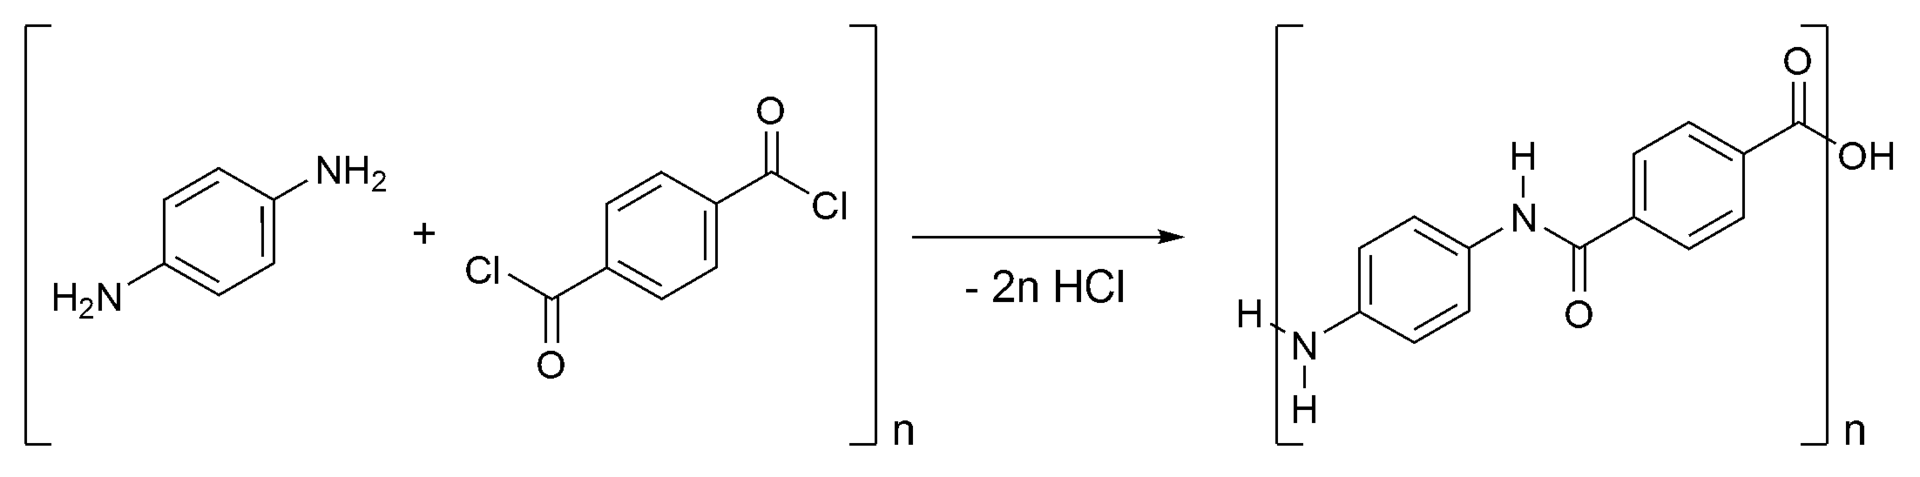
\includegraphics[scale=0.215]{Schema/Kevlar_chemical_synthesis.png}

Le sous-produit de cette réaction est de l'acide chlorhydrique, \ce{HCl}. La présence de cet acide en solution pourrait provoquer des réactions de corrosion et endommager du matériel. Il est donc nécessaire d'introduire des bases (généralement des sels de lithium et carbone) pour neutraliser l'acidité.

Après cette étape, la solution à pris la forme d'une masse visqueuse semblable à du gel. Dans cette masse, il pourrait y avoir des sels insolubles en plus de la fibre voulue. Il faut donc les éliminer avant de continuer le processus.
		
\section{Filage}
	
A la sortie de la première étape, les fibres sont alignées aléatoirement. Cependant, la Kevlar à un comportement nématique, comme un cristal liquide. C'est-à-dire que les fibres ont tendance à s'aligner dans la même direction, par petits paquets, il y a un certain degré d'ordre naturel. En augmentant la concentration, le degré d'aignement augmente mais n'est pas encore parfait.

\begin{center}
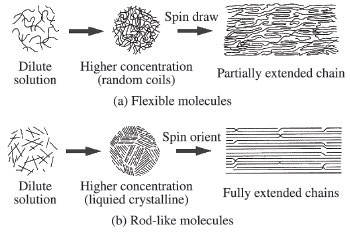
\includegraphics[scale=0.72]{Schema/kevlar_1.jpg}
\end{center}

Pour remédier à celà vient la deuxième étape. Les fibres sont filées, lors d'un processus de filage humide. Les fibres sont dissoutes dans de l'acide sulfurique, H$_2$SO$_4$, et la solution passe sous pression (pour augmenter la concentration) par de très petits orifices (afin d'aligner le plus possible les fibres). Le dispositif est une filière. Lors du passage de la solution à travers les minuscules trous de la filière, les fibres s'alignent dans une même direction et le résultat est ensuite refroidi dans de l'eau froide. 

\clearpage
\section{Flowsheet}

	%Définir les formes
	\tikzstyle{block} = [rectangle, draw, fill=blue!20,text width=14em, text badly centered, rounded corners, minimum height=4em, minimum width=23em, node distance=3cm] %Etape
	\tikzstyle{line} = [draw, ->,>=latex] %Flèche
	\tikzstyle{inn} = [ draw, ellipse,fill=green!60, minimum height=2em] %Entrée
	\tikzstyle{outt} = [midway, draw, ellipse,fill=red!60, node distance=3cm, minimum height=2em] %Sortie
	\tikzstyle{inout} = [midway, draw, ellipse,shade, top color = red!70, bottom color = green!70, node distance=3cm, minimum height=2em] %Entrée/Sortie
	\tikzstyle{values} = [rectangle, draw, fill = gray!20] %Valeur
	\tikzstyle{final} = [midway, diamond, draw, fill=yellow!60, text width=4.5em, text badly centered, node distance=3cm, inner sep=0pt] %Produit final


\begin{center}
	\scalebox{0.95}{
	\begin{tikzpicture}
	    %Place nodes
	    
	    %Première étape : polymérisation 
	    \node[block] (Pol)at(0,13) {\textbf{Polymérisation}
	    $$\ce{[C_6H_4(NH_2)_2 + C_8H_4Cl_2O_2]_n} $$ 
	    $$\ce{->[\ce{-2 n HCl}]}$$
	    $$\ce{[-CO-C_6H_4-CO-NH-C_6H_4-NH-]_n} $$
	    };
	    
	    %Deuxième étape : filage
	    \node[block] (Fil)at(0,6) {\textbf{Filage} 
	    \ce{[-CO-C_6H_4-CO-NH-C_6H_4-NH-]_n} \\
	    $\downarrow$ \\
	    Kevlar
	    };
	
	    \node (in1)at(-4,19) {}; %Premier réactif
	    \node (in2)at(4,19) {};  %Deuxième réactif
	    \node (out1)at(9,13) {}; %Rejet de HCl
	    	\node (pfinal)at(0,0) {};  %Produit final
	    	\node[values] (outtt)at(6.46,13.75) {$306,723\kilogram = 8,404\kilo\mole$}; %Valeurs sur HCl
	    		    	
	    % Draw edges
	    
	    %Premier réactif
	    \path [line] (in1) -- node[inn] {\ce{C_6H_4(NH_2)_2}} node[values, near start] {$453,782\kilogram = 4,202\kilo\mole$} (Pol); 
	    %Deuxième réactif
	    \path [line] (in2) -- node[inn] {\ce{C_8H_4Cl_2O_2}} node[values, near start] {$852,941\kilogram = 4,202\kilo\mole$}(Pol); 
	    %Entre les deux étapes
	    \path [line] (Pol) -- node[inout] {\ce{[C_6H_4(NH_2)_2 + C_8H_4Cl_2O_2]_n}} node[values, near start] {$1000\kilogram = 4,202\kilo\mole$} (Fil); 
	    %Rejet de HCl
	    \path [line] (Pol) -- node[outt] {\ce{HCl}} (out1); 
	    %Produit final
	    \path [line] (Fil) -- node[final] {\textbf{Kevlar}} node[values, pos = 0.8] {$1000 \kilogram = 4,202\kilo\mole$} (pfinal);  

	\end{tikzpicture} }
\end{center}
